%! Author = giaco
%! Date = 16/05/2024

\chapter{Background}
\label{ch:background}
In this chapter, we provide a brief overview of the main concepts that are necessary to understand the work presented in this thesis.
First of all, we start by introducing the concept of Machine Learning and Deep Learning in~\ref{sec:machine_learning}.
Then, in~\ref{sec:rl} we will talk in depth about one specific kind of learning paradigm, i.e.\ Reinforcement Learning, and in~\ref{sec:drl} we will talk about Deep Reinforcement Learning which is instead the main focus of this work.

\section{Machine Learning}
\label{sec:machine_learning}
% image examples https://www.geeksforgeeks.org/types-of-machine-learning/

Machine Learning, Fig. \ref{fig:ml_hierarchy}, is the branch of Artificial Intelligence that focuses on developing models and algorithms that let computers learn from data and improve from previous experience without being explicitly programmed for every task.
In simple words, ML teaches the systems to think and understand like humans by learning from data.
ML finds application in many fields, including natural language processing~\citep{devlin2018bert}, computer vision~\citep{he2016deep}, speech recognition~\citep{hinton2012deep}, email filtering~\citep{carreras2001boosting}, medicine~\citep{esteva2017dermatologist}, and many more

There are several types of ML family of algorithms, each with its characteristics and applications.
Some of the main types are Supervised Learning~\citep{kotsiantis2007supervised}, Unsupervised Learning~\citep{hastie2009elements}, Self-Supervised Learning~\citep{balestriero2023cookbook}, and finally Reinforcement Learning~\citep{sutton1998introduction}, Fig.\ref{fig:ml_types}
A subset of ML is Deep Learning (DL)~\citep{lecun2015deep}, which focuses on training neural networks with many layers.

We will talk about the different kinds of learning algorithms and DL in the following subsection, while since RL is the focus of this work we will dedicate a separate section.




\begin{figure}[ht]
    \begin{subfigure}[b]{0.45\textwidth}
        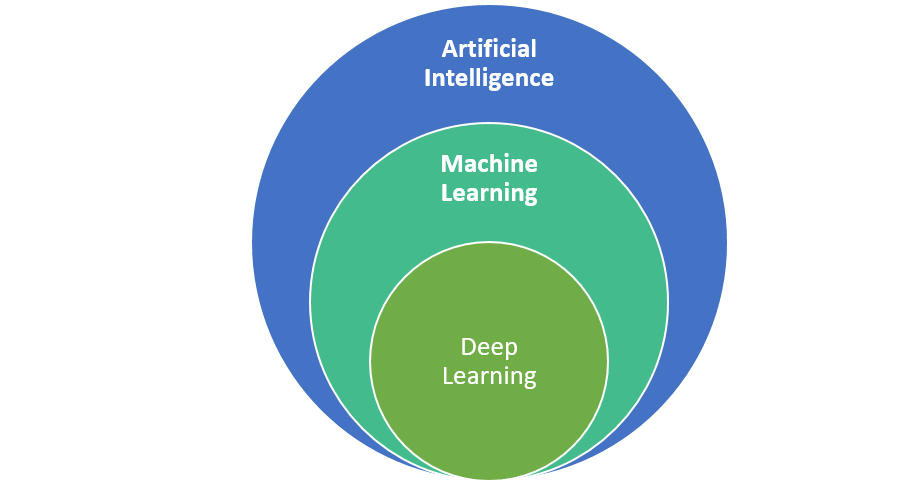
\includegraphics[width=\textwidth]{images/background/ai_ml_dl}
        \caption{\texttt{Artificial Intelligence hierarchy.}}
        \label{fig:ml_hierarchy}
    \end{subfigure}
    \hfill
    \begin{subfigure}[b]{0.45\textwidth}
        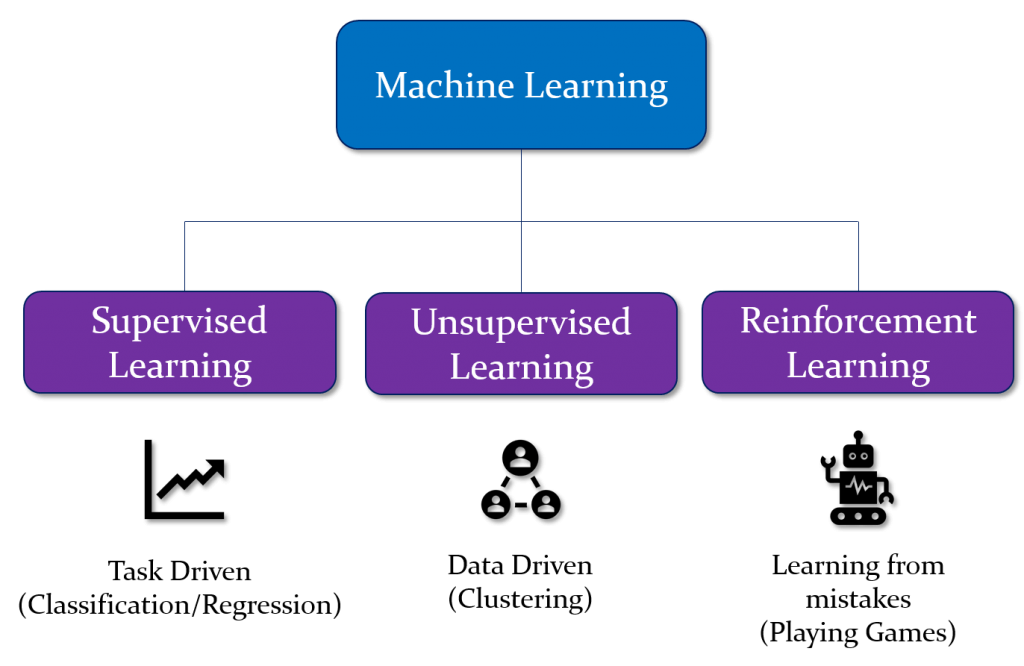
\includegraphics[width=\textwidth]{images/background/ML_Types}
        \caption{\texttt{Some Families of ML algorithms.}}
        \label{fig:ml_types}
    \end{subfigure}
    \hfill
    
\end{figure}








\subsubsection{Supervised Learning}
\label{subsubsec:supervised_ml}
%intro
Supervised Learning is a branch of ML where the model learns from the provided examples under human supervision.
In this context, models are equipped with \textit{labeled} data, meaning that each training example is paired with an output label.
The goal is to learn a mapping function from inputs to outputs that can be used to predict the target for new, unseen inputs.
The process of training a supervised learning model consists of two main phases: training and testing.
During the training phase, the algorithm searches for patterns in the data that can be used to make predictions.
After the training phase, the model can receive in input new unseen data and determine which label it belongs to, this is called the testing phase.

%example
For example, given a dataset of pairs consisting of flower images and their labels representing the flower species, we refer to this as training data or training set.
The aim is to train a model that learns to predict the species of a flower given its image, based on the patterns learned from the training data like color, shape, and size.
When the model outputs the predicted species of a flower image, we can compare it with the true label to evaluate the model's performance.
The learning process is iterative, and the model is updated based on the errors made during the training phase.
If the predicted species is the same as the true label, the model has made a correct prediction, and it does not need to be updated, otherwise, it has made an incorrect prediction, and we need to update its parameters in order to obtain the correct prediction.
Once the model is trained such that to recognize most of the species of the flowers in the training set, it can be used to predict the species of a new flower image that was not present in the training set.


%categories
There are two main categories of supervised learning that are:
\begin{itemize}
    \item Classification - The goal is to predict a discrete label.
    For example, classifying emails as spam or not spam, or recognizing handwritten digits.
    Classification algorithms learn how to map the input features to one of the predefined classes.

    \item Regression - The goal is to predict a continuous value.
    For example, predicting the price of a house given its features, or the temperature for a given day.
    Regression algorithms learn to map the input features to a continuous numerical value.

\end{itemize}

Over the years, many algorithms have been developed to solve supervised learning tasks, including Linear Regression~\citep{james2013introduction}, Support Vector Machines~\citep{cortes1995support}, Decision Trees~\citep{breiman2017classification}, Naive Bayes~\citep{mccallum1998comparison}, and Neural Networks~\citep{lecun1998gradient}.

%pros and cons
Supervised Learning models can have high accuracy when they are trained on a huge amount of quality labeled data.
Also, they can be used as pre-trained models, which saves time and resources when developing new models from scratch.
Moreover, many supervised learning models like decision trees, are interpretable, meaning that it is possible to understand how the model makes predictions.
This is very helpful in context like medicine, where it is important to understand the reasons behind the model's predictions.
They have some limitations though, in fact, sometimes they need a huge amount of data to perform well, meaning that in context where there is a lack of data, they may not be the best choice, meanwhile, in context where there is a huge amount of data, they can be time-consuming to process all the data.
Also, they may suffer from \textit{overfitting} problem, which means that the model learns the training data too well, and it is not able to generalize on unseen data.


\subsubsection{Unsupervised Learning}
\label{subsubsec:unsupervised_ml}
%intro
Unsupervised Learning paradigm is the opposite of Supervised Learning.
It is a technique in which an algorithm discovers patterns and relationships using unlabeled data, i.e.\ it does not require labeled data as target outputs.
The primary goal of Unsupervised learning is to discover hidden patterns, similarities, or clusters within the data, which can then be used for various purposes, such as data exploration, visualization, dimensionality reduction, and more.

%example
For example, given a dataset of customer purchase history, the goal is to group customers based on their purchasing behavior.
The algorithm will group customers with similar purchasing behavior into clusters, and this information can be used to target specific groups of customers with personalized marketing campaigns.

%categories
The main categories of unsupervised learning are:
\begin{itemize}
    \item Clustering - This is the process of grouping data points into clusters based on their similarities.

    \item Association Rule learning - It is a method used for finding relationships between variables in a large database.
    A typical example of the Association Rule is the Market Basket Analysis which determines the set of items that occur together like people who buy a specific item also tend to purchase another item.

\end{itemize}

Many algorithms have been developed through the years for clustering applications like K-means~\citep{macqueen1967some}, Hierarchical Clustering~\citep{johnson1967hierarchical}, or DBSCAN~\citep{ester1996density}.
Also, there are algorithms that use unsupervised learning for dimensionality reduction like PCA~\citep{jolliffe1986principal}.
Finally, for association rule learning, there are algorithms like Apriori~\citep{agrawal1994fast}.


%pros and cons
Unsupervised Learning is really helpful in discover hidden patterns and relationships when labels for data are not available.
But it has some limitations, in fact, it is difficult to evaluate the performance of the model since there are no labels to compare the output with.



\subsubsection{Self-Supervised Machine Learning}
\label{subsubsec:semisupervised_ml}
%intro
Self-supervised Learning paradigm falls in between supervised and unsupervised learning.
As the name suggests, it is a technique where the model learns from the data itself without human supervision.
The training process is divided into two phases: pre-training and fine-tuning.
In the pre-training phase, the model learns to solve a pretext task, which consists of generating labels from the data itself.
This means that the model learns to extract useful feature representations from the data.
In the fine-tuning phase, the extracted features are used to solve the downstream task, for example, classification or regression in a supervised learning setting.


%example
For example, in the context of computer vision, given a dataset of images that have one part obscured or missing, the model can be trained to predict the missing part.
This is a pretext task.
Then, the same model used for the pretext task can be fine-tuned on a downstream task like image classification or object detection.

In the literature, there are many works that use self-supervised learning for various tasks, including image classification~\citep{chen2020simple}, object detection~\citep{he2020momentum}, and natural language processing~\citep{devlin2018bert, radford2018improving}.


%pros and cons
Self-supervised learning is really helpful when labeled data is missing, or difficult to obtain.
It can be used to pre-train models on large amounts of unlabeled data and then fine-tune them on smaller labeled datasets.
This is really helpful in the context of transfer learning, where the model learns from one task and then applies the knowledge to another task.
But it has some limitations, in fact, it requires a lot of computational resources and time to train the model on large amounts of data, and it may not perform well on tasks that are very different from the pretext task.

\subsubsection{Deep Learning}
\label{subsubsec:dl}
In recent years, deep learning has gained a lot of attention and has been successful in many fields.
It can be used in supervised, unsupervised, and self-supervised learning tasks. It focuses on training neural networks with many layers, where each layer is responsible for extracting features from the input data at different levels of abstraction.

In particular, a Neural Network (NN) is an Artificial Intelligence technique that draws inspiration from the functioning of the human brain.
Every NN consists of layers of interconnected nodes, which are called neurons.
A neuron is a computational unit that takes multiple inputs and, to produce an output, a weighted summation of the inputs for some weights is computed.
Also, neurons have an activation function that decides whether a neuron should be activated or not.
Activation functions can be linear or non-linear functions, and they are used to introduce non-linearity in the model, which allows the model to learn more complex patterns in the data rather than linear ones.
Examples of non-linear activation functions are the Sigmoid, the ReLU, and the Hyperbolic Tangent function.

In specific, the computation of a neuron can be expressed as:

\begin{equation}
    \dot{y} = f(\sum_{i=1}^{n} w_i x_i + b)\label{eq:neuron}
\end{equation}

Where $y$ is the output of the neuron, $f$ is the activation function, $w_i$ are the weights, $x_i$ are the inputs, and $b$ is the bias term.
Fig. \ref{fig:single_neuron} shows a picture of a single neuron.



\begin{figure}[ht]
    \begin{center}
        \fbox{\rule[-.5cm]{0cm}{4cm} \rule[-.5cm]{4cm}{0cm}}
    \end{center}
    \caption{Image of a single neuron.}
    \label{fig:single_neuron}
\end{figure}


It is possible to see a NN as a composition of multiple neurons, where the output of one neuron is the input of the next one.
We define \textbf{Multilayer Perceptron} (MLP) as a sequential model that is composed of multiple layers of neurons.
We have an \textit{input layer}, which is responsible for receiving the input data, one or more \textit{hidden layers}, that are responsible for processing the data in a way that encodes the information in a latent space, and finally an o\textit{utput layer}, which is responsible for producing the output information.
In specific, we talk about \textit{feed-forward neural networks}, when the information flows from the input layer to the output layer without any feedback connections, and we talk about \textit{fully-connected neural networks} when each neuron in a layer is connected to every neuron in the next layer.
The mathematical representation of a feed-forward neural network is expressed in Eq. \ref{eq:nn}, while Fig. \ref{fig:nn} shows a picture of a feed-forward neural network.


\begin{equation}
    \hat{y} = f_n(f_{n-1}(\dots f_1(\sum_{i=1}^{n} w_i x_i + b_1) \dots + b_{n-1}) + b_n)
    \label{eq:nn}
\end{equation}


\begin{figure}[ht]
    \begin{center}
        \fbox{\rule[-.5cm]{0cm}{4cm} \rule[-.5cm]{4cm}{0cm}}
    \end{center}
    \caption{Image of a neural network.}
    \label{fig:nn}
\end{figure}


The process of learning the weights relies on the \textbf{backpropagation} algorithm \citep{rumelhart1986learning} that consists of two main steps: forward pass and backward pass.

Suppose we are in a supervised learning setting, and we have a dataset of input data $x$ and labeled output $y$, the output data is referred to as ground-truth.
In the forward pass, the input data is passed through the network and the predicted output $\hat{y}$ is computed.
Then, considering the output of the network, the error is computed using a loss function which is a distance metric and measures the difference between the predicted output and the ground-truth.
A typical loss function is the Mean Squared Error (MSE) which is defined as:

\begin{equation}
    MSE = \frac{1}{n} \sum_{i=1}^{n} (y_i - \hat{y}_i)^2
\end{equation}

The backward pass consists of propagating the error back through the network, from the output layer to the input one, and it is responsible for updating the weights to minimize the error between the predicted output and the ground-truth.
Weights are updated using the \textit{gradient descent algorithm}, which is an optimization method that iteratively updates the weights in the direction that minimizes the loss function.
In neural networks, backpropagation is implemented using the chain rule to compute the gradients of the loss function with respect to the weights. 
Decomposing the computation of the gradient of the loss into simpler computations makes the computation of the gradients more efficient and allows the training of deep neural networks.
In Fig. \ref{fig:gradient_descent} it is possible to see an image that represents the gradient descent method, while in Algorithm \ref{alg:gradient_descent} we provide the pseudocode of the gradient descent algorithm.

\begin{algorithm}
\caption{Gradient Descent Algorithm}\label{alg:gradient_descent}
\begin{algorithmic}
    \State Initialize the weights $w$ randomly
    \While{not converged}
        \State Compute the predicted output $\hat{y}$
        \State Compute the loss $L$
        \State Compute the gradient of the loss w.r.t the weights $\nabla_w L$
        \State Update the weights $w = w - \alpha \nabla_w L$
    \EndWhile
\end{algorithmic}
\end{algorithm}





\begin{figure}[ht]
    \begin{center}
        \fbox{\rule[-.5cm]{0cm}{4cm} \rule[-.5cm]{4cm}{0cm}}
    \end{center}
    \caption{Image of loss and gradient steps.}
    \label{fig:gradient_descent}
\end{figure}



In the literature, multi-layered neural networks are referred to as Deep Neural Networks (DNNs), and the process of training them is called Deep Learning.
One of the most successful architectures in deep learning is the Convolutional Neural Network (CNN), which is commonly used in computer vision tasks.
CNNs are composed of:

\begin{itemize}
    \item convolutional layers, which applies a set of kernels to the input data to extract features.
    Each kernel extracts a different feature, and the output of a convolutional layer is a set of feature maps.
    \item activation functions, which introduce non-linearity in the model.
    \item pooling layers, which reduce the dimensionality of the data by reducing the size of feature maps.
    A typical example of pooling is \textit{max-pooling}, which takes the maximum value in a window of the feature map.
    \item fully connected layers, which take as input the extracted features and make the predictions.
\end{itemize}

Fig. \ref{fig:cnn} shows a picture of a CNN architecture.

\begin{figure}[ht]
    \begin{center}
        \fbox{\rule[-.5cm]{0cm}{4cm} \rule[-.5cm]{4cm}{0cm}}
    \end{center}
    \caption{Image of a CNN.}
    \label{fig:cnn}
\end{figure}


%talk about feed forward nn vs cnn?

\section{Reinforcement Learning}
\label{sec:rl}

Reinforcement Learning is a paradigm of ML works in a way that mimics the trial-and-error learning process that humans use to achieve their goals.
The principal elements that form RL are: the agent, the environment, and the reward signal.

The environment represents the world where the agent lives.
The agent instead is the learner that interacts with it, and for each action that the agent makes, it obtains a reward that usually is a scalar number.
RL focuses on training agents to make sequences of decisions in the environment to maximize the cumulative reward.
In particular, in RL, there is no supervision.
The only feedback that the agent receives is the reward signal that indicates how well it is doing and should be informative enough to let the agent learn the optimal behavior.
Fig. \ref{fig:rl} shows a picture of the RL paradigm.


\begin{figure}[ht]
    \begin{center}
        \fbox{\rule[-.5cm]{0cm}{4cm} \rule[-.5cm]{4cm}{0cm}}
    \end{center}
    \caption{RL sample image with environment, observation, agent, action, reward.}
    \label{fig:rl}
\end{figure}


Environments can be \textit{fully observable} when the agent has access to the complete state of it, or \textit{partially observable} when the agent has only partial information of the full environment.
Specifically, in the presence of fully observable environments, we formalize the RL problem as a Markov Decision Process (MDP), which is a tuple $(S, A, P, R, \gamma)$, where:
\begin{itemize}
    \item $S$ is the set of states that the agent can be in.
    \item $A$ is the set of actions that the agent can take.
    \item $P$ is the transition probability function, which defines the probability of transitioning from one state to another given an action.
    \item $R$ is the reward function, which defines the reward that the agent receives when transitioning from one state to another.
    \item $\gamma$ is the discount factor, which determines the importance of future rewards.
    If it is close to 0, the agent will consider only immediate rewards, while if it is close to 1, the agent will consider future rewards.
\end{itemize}

It is possible to define the return of an agent in an MDP as the sum of discounted reward from a specific timestep t.
In particular:
\begin{equation} \label{eq:return}
    G_t = R_{t+1} + \gamma R_{t+2} + \gamma^2 R_{t+3} + \dots = \sum_{k=0}^{\infty} \gamma^k R_{t+k+1}
\end{equation}

The principal components of an RL agent are three and in order are: the policy $\pi$, the value function $v$, and the model $m$.
We will now explain them one by one.

The policy defines the behavior of the agent, it is a mapping from states to actions.
Policy can be deterministic if it maps states to a single action, or stochastic if it maps states to a distribution over all possible actions.
The policy can be represented as a table, a function, or a neural network, and in the context of MDPs, the policy is defined in Eq. \ref{eq:policy} and it is the probability of taking action $a$ considering to be in state $s$.

\begin{equation} \label{eq:policy}
    \pi(a|s) = P(a|s)
\end{equation}



The value function estimates the expected return that the agent can achieve starting from a given state and following a given policy $\pi$.
It is used to evaluate how good a state is, and it is defined as:

\begin{equation} \label{eq:value_function}
    v_{\pi}(s) = \E_{\pi}[R_{t+1} + \gamma R_{t+2} + \gamma^2 R_{t+3} + \dots | S_t = s] = \E_{\pi}[G_t | S_t = s]
\end{equation}

This is also called the \textbf{state-value function}.
It exists an equivalent function that estimates the expected return that the agent can achieve starting from a given state, taking a specific action, and then following a given policy $\pi$.
This is called the \textbf{action-value function}, and it is defined in Eq. \ref{eq:action_value_function}.
Value functions too can be represented as tables, functions, or neural networks.

\begin{equation} \label{eq:action_value_function}
\begin{split}
    q_{\pi}(s, a) = \E_{\pi}[R_{t+1} + \gamma R_{t+2} + \gamma^2 R_{t+3} + \dots | S_t = s, A_t = a] \\
    = \E_{\pi}[G_t | S_t = s, A_t = a]
\end{split}
\end{equation}


The model is used to predict what the environment will do next.
If an agent knows the model, means that it knows what will be the next state given the current state and action (Eq. \ref{eq:next_state}), and also, it can predict the next reward given the current state and action (Eq. \ref{eq:next_state}). 

\begin{equation} \label{eq:next_state}
    P_{s, s'}^a = P(S_{t+1} = s' | S_t = s, A_t = a)
\end{equation}

\begin{equation} \label{eq:next_reward}
    R_s^a = \E[R_{t+1} | S_t = s, A_t = a].
\end{equation}

In RL, we have two fundamental tasks, \textit{prediction} and \textit{control}. 
Prediction involves estimating the value function of an unknown MDP, while control involves finding the optimal policy.
The concept of learning in RL is based on the \textbf{Bellman Equations}, which form the basis for many RL algorithms and are divided into two main categories: the \textit{Bellman Expectation Equations} and the \textit{Bellman Optimality Equations} which we will explain now.


To estimate the goodness of a state, i.e. the value functions, we can use the Bellman Expectation Equations for the state-value function and the action-value function, which provides a recursive relationship between the value to be in a state at a specific time and the expected return starting from the next state.

Bellman Expectation for the state-value function is defined in Eq. \ref{eq:bellman_state_value} where the expected return is decomposed into the immediate reward and the discounted value of the next state, and then we marginalize over all the possible actions to obtain the expected value of the state in terms of the action-value function.

\begin{equation} \label{eq:bellman_state_value}
    v_{\pi}(s) = \E_{\pi}[R_{t+1} + \gamma v_{\pi}(S_{t+1}) | S_t = s] = \sum_{a \in A} \pi(a|s)q_{\pi}(s, a)
\end{equation}

Similarly, the Bellman Expectation for the action-value function is defined in Eq. \ref{eq:bellman_action_value}, where the expected return is decomposed into the immediate reward and the discounted value of the next state-action pair, and then we marginalize over the next states to obtain the expected value of the action in terms of the state-value function.

\begin{equation} \label{eq:bellman_action_value}
\begin{split}
    q_{\pi}(s, a) = \E_{\pi}[R_{t+1} + \gamma q_{\pi}(S_{t+1}, A_{t+1}) | S_t = s, A_t = a] \\
    = R_s^a + \gamma \sum_{s' \in S} P_{s, s'}^a v_{\pi}(s')
    \end{split}
\end{equation}

Now we notice that the Bellman Equation for the state-value function defined in Eq. \ref{eq:bellman_state_value} can be rewritten substituting the action-value function in it, obtaining:

\begin{equation}
    v_{\pi}(s) = \sum_{a \in A} \pi(a|s)(R_s^a + \gamma \sum_{s' \in S} P_{s, s'}^a v_{\pi}(s'))
\end{equation}

Similarly, the Bellman Equation for the action-value function defined in Eq. \ref{eq:bellman_action_value} can be rewritten substituting the state-value function in it, obtaining:

\begin{equation}
    q_{\pi}(s, a) = R_s^a + \gamma \sum_{s' \in S} P_{s, s'}^a \sum_{a' \in A} \pi(a'|s')q_{\pi}(s', a')
\end{equation}



A policy $\pi$ is defined to be better than or equal to a policy $\pi'$ if an agent, following the policy $\pi$ is expected to obtain a return that is greater than or equal to the one obtained by an agent following the policy $\pi'$.
%In other words pi >= pi'  and only if v_pi(s) >= v_pi'(s) for all s.
There is always at least one policy that is better than or equal to all other policies.
This is an \textit{optimal policy}.
There may be more than one optimal policy, but we denote all the optimal policies by $\pi^*$.
For finding the optimal policy $\pi^*$, we can use the \textbf{Bellman Optimality Equations} both for the state-value function and the action-value function.
Supposing that we have the optimal action-value function $q_*(s, a)$, i.e. a function that estimates correctly the expected return,
we can obtain the optimal policy simply by choosing always the action that maximizes the action-value function in a given state:

\begin{equation}
    \label{eq:optimal_policy}
    \pi^*(a|s) = \begin{cases}
        1 & \text{if } a = \arg\max_{a} q_*(s, a) \\
        0 & \text{otherwise}
    \end{cases}
\end{equation}


So we can define the Bellman Optimality Equation to find the optimal state-value function as follows:

\begin{equation} \label{eq:optimal_state_value}
    v_*(s) = \max_{a} q_*(s, a) = \max_{a} R_{t+1}^a + \gamma \sum_{s'} P_{s, s'}^a v_*(s')
\end{equation}

The Bellman Optimality Equation to find the optimal action-value function is as follows:

\begin{equation} \label{eq:optimal_action_value}
    q_*(s, a) = R_s^a + \gamma \sum_{s'} P_{s, s'}^a v_*(s') = R_s^a + \gamma \sum_{s'} P_{s, s'}^a \max_{a'} q_*(s', a')
\end{equation}


Solving the Bellman Equations means finding the optimal policy.


In the world of RL, there exist many algorithms that can be distinguished into model-based algorithms, where the agent knows the environment, and model-free algorithms, where the agent does not need a model of the environment.
Within model-free RL, some algorithms focus on optimizing the value function (value-based RL), other tries to optimize the policy (policy-based RL), and some of them both (Actor-Critic).
In the following sections, we will explore briefly model-based and model-free RL algorithms, we will talk about how to approximate the value functions and the policy using neural networks.
We will also talk about some of the most famous RL algorithms, including \textit{Q-learning}, \textit{Deep Q-Learning}, and \textit{Proximal Policy Optimization}.


\subsection{Model Based Reinforcement Learning}
\label{subsec:model_based_rl}
Model-based RL is more like planning, agents build a model of the environment and then use it to plan their actions.
Model-based RL algorithms are based on the Bellman Equations and include algorithms like \textbf{Policy Iteration} \citep{howard1960dynamic} and \textbf{Value Iteration} \citep{bellman1966dynamic}.

Policy Iteration is an algorithm that computes the optimal policy by iteratively applying the \textit{Bellman Expectation Equation}.
It alternates between policy evaluation, which computes the value function for a given policy using the Bellman Expectation Equation, and policy improvement, which computes the optimal policy given the value function acting greedily i.e.\ choosing the action that maximizes the action-value function in a given state.
It is guaranteed to converge to the optimal policy, but it is computationally expensive.

Value Iteration is an algorithm that computes the optimal value function by iteratively applying the \textit{Bellman Optimality Equation}.
There is no explicit policy here, its goal is to find an optimal policy $\pi$ so, at each iteration, it computes the value function for all states, trying to improve the estimate of it 
It is guaranteed to converge to the optimal value function.

Both Policy Iteration and Value Iteration use dynamic programming approaches to solve the Bellman Equations.

\subsection{Model Free}
\label{subsec:model_free_rl}
In the model-free approach, a model of the environment is not needed.
Agents learn the optimal policy without explicitly learning the dynamics of the environment so there is no knowledge of the transition probabilities and the reward function.
Agents learn by interacting with the environment and observing the rewards.
We will now explore the \textit{control} problem, and we will talk about an approach to solve it, i.e.\ Q-learning.


Model-free control RL algorithms can be divided into two main categories: \textbf{on-policy} and \textbf{off-policy} algorithms.
On-policy means that the agent learns the policy $\pi$ while following the current policy, so it learns from experience sampled from $\pi$.
Off-policy means that the agent learns the policy $\pi$ while following a different policy $\mu$.
This is very helpful in the context of \textit{learning from imitation} or reusing experiences.

In the context of Off-policy learning, a well-known algorithm is \textbf{Q-learning}.
Q-learning learns the optimal action-value function by iteratively applying the Bellman Optimality Equation.
Since a model of the environment is not known, it is not possible to compute the expected value of the next state, so Q-learning uses the concept of \textit{Temporal Difference} (TD) learning, which consists of updating the action-value function by taking the difference between the current estimate of the value function on a specific state, and the target estimate of the value function.
This is called \textit{TD error}.
The target, in this case, is defined as the immediate reward plus the maximum action-value function of the next state.
This is because we act greedily, so we choose the action that maximizes the action-value function in the next state.

In Eq. \ref{eq:q_learning} we show the Q-learning update rule where the TD error is multiplied by the learning rate $\alpha$ and added to the current estimate.

\begin{equation} \label{eq:q_learning}
    Q(S_t, A_t) \leftarrow Q(S_t, A_t) + \alpha [R_{t+1} + \gamma Q(S_{t+1}, a) - Q(S_t, A_t)]
\end{equation}

We report also the pseudocode of the Q-learning algorithm in Algorithm \ref{alg:q_learning}.


\begin{algorithm}
\caption{Q-Learning Algorithm}\label{alg:q_learning}
\begin{algorithmic}
\State Initialize $Q(s, a)$,  $\forall s \in S, a \in A$ arbitrarily and $Q(\text{terminal state}, \cdot) = 0$
\For{each episode}
    \State Initialize $S$
    \For{each step of the episode}
        \State Choose $A$ from $S$ using policy derived from $Q$
        \State Take action $A$, observe $R$, $S'$
        \State $Q(S, A) \leftarrow Q(S, A) + \alpha [R + \gamma \max_{a'} Q(S', a') - Q(S, A)]$
        \State $S \leftarrow S'$
    \EndFor
\State Until S is terminal
\EndFor




\end{algorithmic}
\end{algorithm}



\section{Deep Reinforcement Learning}
\label{sec:drl}
Till now we have seen how to solve the RL problem using tabular methods, i.e.\ the value function scores and the policy are represented as tables.
These methods are intractable when the state space is large or continuous.
In this section, we will talk about how value functions and policies can be predicted using neural networks as universal function approximators.
The combination of DL techniques and RL is called Deep Reinforcement Learning (DRL) \citep{mnih2015human}.

DRL has been successful in many tasks, including playing video games, controlling robots, and optimizing complex systems.
Both prediction and control problems can be addressed using DRL.
We will make distinctions between value function approximation and policy function approximation talking about policy gradient methods. 
We will provide an overview of two of the most famous DRL algorithms, i.e.\ \textbf{Deep Q-Learning} (DQL) and \textbf{Proximal Policy Optimization} (PPO).


\subsection{Value Function Approximation}
\label{subsec:value_function_approx}
In the context of DRL, the value function can be approximated using different types of approaches, including linear function approximation, decision tree and in particular neural networks.

The goal is to find a parameter vector \textbf{w} that minimizes the MSE between the predicted value function $\hat{v}(s,\textbf{w})$ and the true value function $v_\pi(s)$.
This can be done using the \textit{Gradient Descent} algorithm and can be accomplished in a batch or online way.
The convergence though is not guaranteed for all algorithms and depends on the choice of the value function approximator (linear or non-linear).

Regarding batch methods, a well-known algorithm is the Deep Q-Learning.
It is based on the Q-learning algorithm, but it uses neural networks to approximate the action-value function
Also, it uses the concept of \textit{experience replay} and $\epsilon$-greedy policy.
Going in order, actions are chosen using a $\epsilon$-greedy policy, which means that with probability $\epsilon$ the agent chooses a random action, and with probability 1-$\epsilon$ the agent acts greedily and chooses the action that maximizes the action-value function.
The experience replay instead, consists of storing the agent's experiences in a replay buffer, which we call \textit{D}.
The buffer will contain the agent's transitions, which are tuples consisting of $(s, a, r, s')$, where $s$ is the initial state, $a$ is the action taken, $r$ is the reward received, and $s'$ is the next state.
To update the action-value function, the agent samples a batch of transitions from the replay buffer, this transitions represent the ground-truth, and are used to compute the TD error.

The neural networks involved in the DQL algorithm are two, the online network and the target network, and they are called Deep Q-Networks (DQN).
The online network is used to predict the action-value function, while the target network is used to compute the target action-value function.

The loss function is defined in Eq. \ref{eq:dqn_loss} and it is the MSE between the predicted action-value function and the target action-value function.
In the formula, $D$ is the replay buffer, $\textbf{w}$ are the weights of the neural network, and in specific $\textbf{w}^-$ are the weights of the target network, which are updated less frequently than the weights of the online network.


\begin{equation} \label{eq:dqn_loss}
    L(\textbf{w}) = \E_{(s, a, r, s') \sim D_i} [(r + \gamma \max_{a'} Q(s', a', \textbf{w}^-) - Q(s, a, \textbf{w}))^2]
\end{equation}

The pseudocode of the DQL algorithm is reported in Algorithm \ref{alg:dqn}.

\begin{algorithm}
\caption{Deep Q-Learning Algorithm}\label{alg:dqn}
\begin{algorithmic}
\State Initialize replay buffer $D$
\State Initialize online network $Q$ with random weights $\textbf{w}$
\State Initialize target network $Q^-$ with weights $\textbf{w}^- = \textbf{w}$
\For{each episode}
    \State Initialize $S$
    \For{each step of the episode}
        \State Choose $A$ from $S$ using $\epsilon$-greedy policy
        \State Take action $A$, observe $R$, $S'$
        \State Store transition $(S, A, R, S')$ in $D$
        \State Sample random minibatch of transitions $(s, a, r, s')$ from $D$
        \State Compute target $y = r + \gamma \max_{a'} Q(s', a', \textbf{w}^-)$
        \State Compute loss $L = (y - Q(s, a, \textbf{w}))^2$
        \State Update weights $\textbf{w}$ by minimizing the loss
        \State Every $C$ steps, update target network weights $\textbf{w}^- = \textbf{w}$
        \State $S \leftarrow S'$
    \EndFor
\State Until S is terminal
\EndFor
\end{algorithmic}
\end{algorithm}





\subsection{Policy Gradients}\label{subsec:policy_gradients}
As we have seen, the value function can be approximated using neural networks, but also the policy can be approximated using neural networks.
The goal is, given a policy $\pi(a|s, \textbf{w})$, to find the parameter vector $\textbf{w}$ that maximizes the expected return.
First of all, in Eq. \ref{eq:obj_function} we define the objective function that we want to maximize, where $\pi_w$ is the policy parameterized by $\textbf{w}$, and $S_0$ is the initial state.

\begin{equation} \label{eq:obj_function}
    J(\textbf{w}) = \E_{\pi_w}[\sum_{t=0}^{\infty} \gamma^t R_t | S_0 = s]
\end{equation}

According to the \textbf{Policy Gradient Theorem} \citep{sutton1999policy}, the gradient of the objective function can be expressed as the expected value of the gradient of the log-probability of the action multiplied by the return.
So we can write the policy gradient as in Eq. \ref{eq:policy_gradient}.
In the formula, $\nabla_{\textbf{w}} \log \pi(a|s, \textbf{w})$ is the score function.

\begin{equation} \label{eq:policy_gradient}
    \nabla_{\textbf{w}} J(\textbf{w}) = \E_{\pi_w}[\nabla_{\textbf{w}} \log \pi(a|s, \textbf{w}) Q^{\pi}(s, a, \textbf{w})]
\end{equation}


To compute the score function, Softmax Policy or Gaussian Policy are two common choices.

Policy Gradient methods are effective, but they can be unstable.
In fact, they need a high amount of samples to converge, and they can suffer from high variance, meaning that, for a parameterized policy $\pi(a|s, \textbf{w})$ which returns a distribution over actions, small changes in the policy parameters can lead to large changes in the policy distribution and so in choosing actions.
The changes need to be controlled, so we need to regulate the gradient of the policy.
In this context, \textbf{Natural Policy Gradients} \citep{kakade2001natural} tries to solve this issue.
This, in simple words, means that we want to find the direction in the parameter space that maximizes the expected return, but we want to do it in a way that the changes in the policy are small.


One algorithm that uses Natural Policy Gradients is Proximal Policy Optimization (PPO) \citep{schulman2017proximal}, which works by clipping the policy gradient, so it limits the change in the policy parameters.
The PPO algorithm is based on the idea of alternating between sampling data from the environment and updating the policy.
Its architecture is composed of two neural networks:

\begin{itemize}
    \item \textbf{Policy Network} - It is a network that takes the state of the environment as input and outputs the probability distribution over actions.
    It represents the behavior of the agent.
    \item \textbf{Value Network} - It is a network that takes the state of the environment as input and outputs the value function, so an estimate of the expected return that the agent can achieve starting from a given state.
    Including the value function in the PPO algorithm helps to reduce the variance of the policy gradient.
\end{itemize}

The objective function of PPO changes with respect to one of the policy gradients defined in Eq. \ref{eq:obj_function} in a way that includes a penalty term that clips the gradient.
It is defined in Eq. \ref{eq:ppo_objective}, where $r_t(\textbf{w})$ is the probability ratio between the new policy and the old policy, we want it to be close to 1 as in this way the changes between the policy are small. 
$A_t$ is the advantage function, which is a measure of how good an action is compared to the average action.
Finally, $\epsilon$ is a hyperparameter that controls the clipping of the policy gradient.

\begin{equation} \label{eq:ppo_objective}
\begin{split}
    L(\textbf{w}) = \E_t [\min( r_t(\textbf{w})A_t, \ \text{clip}(r_t(\textbf{w}), 1-\epsilon, 1+\epsilon)A_t)] \\
    r_t(\textbf{w}) = \frac{\pi(a_t|s_t, \textbf{w})}{\pi(a_t|s_t, \textbf{w}_{\text{old}})}
\end{split}
\end{equation}

The pseudocode of the PPO algorithm is reported in Algorithm \ref{alg:ppo}.



In the development of this thesis, we used the PPO algorithm during the training of our agents, and to validate our approach we tested the method also with the DQL algorithm.



\begin{algorithm}
\caption{Proximal Policy Optimization Algorithm}\label{alg:ppo}
\begin{algorithmic}
\State Initialize policy network $\pi(a|s, \textbf{w})$ and value network $V(s, \textbf{w})$
\For{each iteration}
    \For{each epoch}
        \State Collect a batch of data by running the policy in the environment
        \State Compute the advantage function $A_t$
        \State Compute the probability ratio $r_t(\textbf{w})$
        \State Compute the clipped objective function $L(\textbf{w})$
        \State Compute the value function loss $L_v(\textbf{w})$
        \State Update the policy network by minimizing $L(\textbf{w})$
        \State Update the value network by minimizing $L_v(\textbf{w})$
    \EndFor
\EndFor
\end{algorithmic}
\end{algorithm}

